\documentclass[a4paper, oneside]{memoir}% Document class
\usepackage[a4paper]{geometry}			% Margins
\usepackage{lmodern}
\usepackage{graphicx}
\usepackage{float}
\usepackage{listings}
\usepackage[small,compact]{titlesec}	% No 'chapter' in chapter headings.
\graphicspath{{Media/}}					% Directory that holds images.

\titleformat{\chapter}[hang]
{\normalfont\Large\bfseries}{\thechapter}{1em}{\Large}
\titlespacing{\chapter}{0pt}{*0}{*1}

\titleformat{\chapter}{\Huge\bfseries}{\thechapter}{1em}{}
\titleformat{\section}{\LARGE\bfseries}{\thesection}{1em}{}
\titleformat{\subsection}{\Large\bfseries}{\thesubsection}{1em}{}
\titleformat{\subsubsection}{\normalsize\bfseries}{\thesubsubsection}{1em}{}


\author{
  Erik Sidelmann Jensen\\
  \texttt{ejens11@student.aau.dk}
  \and
  Lasse Vang Gravesen\\
  \texttt{lgrave11@student.aau.dk}
  \and
  Dennis Jakobsen\\
  \texttt{djakob11@student.aau.dk}  
}

\title{Data Intensive Systems - Miniproject - Part 1}
\date{}

\begin{document}
	\clearpage\maketitle
	\thispagestyle{empty}
	
	\chapter{DIS Miniproject}
	\section{Task B}
	\begin{itemize}
	\item Sales
	\item Payments
	\item Members
	\item Location
	\end{itemize}
	
	We pick the 'Sales' business process, because it is the most interesting. For that we need to model sales, products, members along with the time and date.
	
	As for granularity, when it comes to sales the time goes down to seconds. We decided to cut it off at minutes, because seconds are not that important. When it comes to members, the granularity goes down to years and there is no more information so that is the only thing that is retained. 
	
	For product it is somewhat possible to add extra levels to the hierarchy, such as category of product like dairy or soda.
	
	The data is reasonable for paying customers and detailed enough to ask valuable questions.
	
	Examples of questions:
	\begin{itemize}
	\item How much is bought at some point during some day?
	\item How does the amount sold change over time?
	\item Which days are the most busy?
	\item When is it best to restock, given low activity?
	\item How much revenue is gained each day, week, month, year?
	\item Which products have changed the most in price from year to year?
	\item Which department or member have spent the most?
	\end{itemize}


	\section{Task C}
	Slowly changing dimensions are not that important.
	
	The business process proposed to be modelled in the data warehouse is the 'Sales' business process. With regards to dimensions we pick out product, time, date, and member because they allow for the most interesting queries. Our granularity with regards to time goes down to minutes across two different dimensions to reduce the amount of rows, with regard to product it only has a name attribute, with regard to member it has balance and year. It might be a good idea to split products into categories, but the data does not directly allow for that and it would have to be done manually based on the name. It might also be a good idea to show if its a special day, like if its a holiday or if a day falls in a vacation.
	
	The schema for the dimensions can be seen below. 
	
	\begin{minipage}{0.45\textwidth}
	\begin{figure}[H]
		\centering
		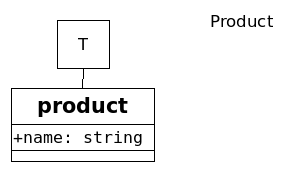
\includegraphics[scale=0.5]{dimensionProduct}
		\label{image:product}
		\caption{The product dimension.}
		\end{figure}
	\end{minipage}
	\begin{minipage}{0.45\textwidth}
	\begin{figure}[H]
	\centering
	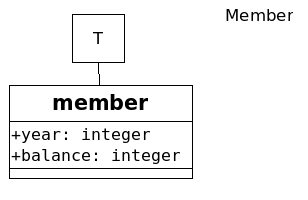
\includegraphics[scale=0.5]{dimensionMember}
	\label{image:member}
	\caption{The member dimension.}
	\end{figure}
	\end{minipage}
	
	\begin{minipage}{0.45\textwidth}
	\begin{figure}[H]
	\centering
	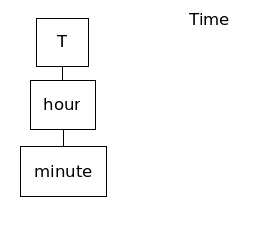
\includegraphics[scale=0.5]{dimensionTime}
	\label{image:time}
	\caption{The time dimension.}
	\end{figure}
	\end{minipage}
	\begin{minipage}{0.45\textwidth}
	\begin{figure}[H]
	\centering
	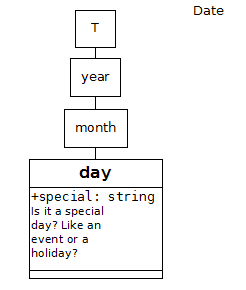
\includegraphics[scale=0.5]{dimensionDate}
	\label{image:date}
	\caption{The date dimension.}
	\end{figure}
	\end{minipage}
	
	The star schema for it can be seen below.  With the schema it is important to note that the dimensions have a surrogate key with a serial integer(it auto increments).
	
	
	\begin{figure}[H]
	\centering
	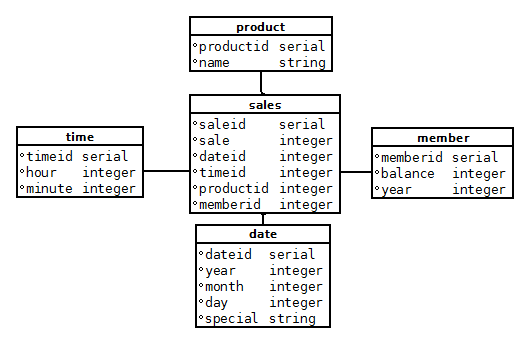
\includegraphics[scale=0.75]{star-scheme}
	\label{image:starschema}
	\caption{The star schema for the data warehouse.}
	\end{figure}
	
	Here is the SQL Table creation text, with some things like serial sequences stripped:
	
	\lstinputlisting[language=SQL]{fklubSimpel.sql}
		
	

\end{document}
